\documentclass{beamer}
\usepackage{hyperref}
\usepackage{color}

\mode<presentation>
{
  \usetheme{default}
  \usecolortheme{default}
  \usefonttheme{default}
  \setbeamertemplate{caption}[numbered]
}

\usepackage[english]{babel}
\usepackage[utf8x]{inputenc}

\title[HRR17]{Steganography}
\author{Peranat Dayananda}
\date{W11 D1}

\begin{document}

\begin{frame}
  \titlepage
\end{frame}

\section{Introduction}

\begin{frame}{What is it?}

\begin{itemize}
  \item Hiding your secret in a way such that no one else knows of its existence
  \item Secret messages, files, etc. are embedded in other seemingly innocuous `hosts' such as documents, pictures, music
\end{itemize}

\begin{figure}
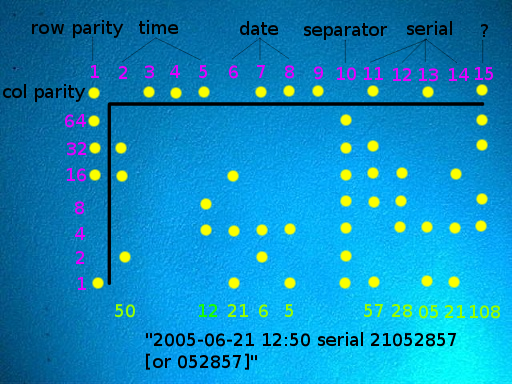
\includegraphics[width=4.5cm]{./printer.png}
\end{figure}

\vskip -.7cm

\begin{block}{Examples}
Your printer prints out tiny dots on every single document, encoding the timestamp, and its serial number to make that document traceable back to you.
\end{block}

\end{frame}

\section{Examples}

\begin{frame}{Simple Case: Hiding a file in a bitmap image}

\begin{itemize}
\item A pixel in a bitmap image is encoded by 3 bytes, each representing the colours red, green, and blue
\end{itemize}

\begin{table}
\centering
\begin{tabular}{l|c|c}
Colour & Value & Binary \\
\hline
Red & 137 & \texttt{10001001}  \\
Green & 44 & \texttt{00101100} \\
Blue & 71 & \texttt{01000111}  \\
\end{tabular}
\caption{Example of a pixel}
\end{table}

\end{frame}

\begin{frame}{Simple Case: Hiding a file in a bitmap image}

\begin{itemize}
\item People probably wouldn't notice a difference if we changed the value of RGB by up to 1 each
\item We can embed our secret file by breaking it up into bits, and then writing each bit onto the least significant bit of each byte in the image
\end{itemize}

\begin{table}
\centering
\begin{tabular}{l|c|c|l}
Colour & Value & Binary & Secret file\\
\hline
Red & 136 & \texttt{1000100 {\color{red} 0}} & $\Leftarrow$ 0\\
Green & 45 & \texttt{0010110 {\color{red} 1}}& $\Leftarrow$ 1\\
Blue & 70 & \texttt{0100011 {\color{red} 0}} & $\Leftarrow$ 0\\
\end{tabular}
\caption{We write the bits of our file onto the least significant bits}
\end{table}

{\quad \Large \href{run:./steg.js}{Demo}}

\end{frame}

\end{document}
